% Pagina originale 5
\pagina{5}
\tit{Minorante e maggiorante}
$m$ è minorante di $A$, $A\ne\varnothing$, se $\forall a\in A:\ m\le a$.
$M$ è maggiorante di $A$, $A\ne\varnothing$, se $\forall a\in A:\ M\ge a$.
\tit{Insieme limitato}
\[A\subset\R\text{ limitato}\iff\begin{cases}\exists M\in\R:\forall a\in A, M\ge a &\text{limitato superiormente (esiste maggiorante)},\\\exists m\in\R:\forall a\in A, m\le a &\text{limitato inferiormente (esiste minorante)}.\end{cases}\]
\tit{Insieme illimitato}
\[A\subset\R\text{ illimitato}\iff
\bigl(\nexists M\in\R:\forall a\in A, M\ge a\bigr)\ \lor\ 
\bigl(\nexists m\in\R:\forall a\in A, m\le a\bigr).\]
\tit{Massimo e minimo}
$m$ è minimo di $A$, $A\ne\varnothing$, se $\exists m\in A$ tale che $\forall a\in A:\ m\le a$.
$M$ è massimo di $A$, $A\ne\varnothing$, se $\exists M\in A$ tale che $\forall a\in A:\ M\ge a$.
\tit{1 --- Unicità del minimo}
Dimostrazione per assurdo. Esistano $m_1,m_2\in A$, con $m_1\ne m_2$, entrambi minimi. Quindi
\[\begin{cases}\forall a\in A:m_1\le a,\\\forall a\in A:m_2\le a\end{cases}\implies
\begin{cases}m_1\le m_2,\\m_2\le m_1\end{cases}\implies\boxed{m_1=m_2!}\]
% Pagina originale 6
\pagina{6}
\tit{Intervallo}
Sia $I\subset\R$. $I$ è intervallo se
\[\forall x,y\in I, x\le y:\quad\forall c\in\R, x\le c\le y\implies c\in I.\]
\tit{Operazioni tra insiemi}
Unione: $A\cup B:=\{x\mid x\in A\lor x\in B\}$.
Intersezione: $A\cap B:=\{x\mid x\in A\land x\in B\}$.
Esclusione: $A\setminus B:=\{x\mid x\in A\land x\notin B\}$.
\tit{Estremo superiore e inferiore}
$A\subset\R$, $A$ limitato inferiormente [rispettivamente superiormente].
\[\R\ni\lambda=\inf A\iff\begin{cases}\forall a\in A:\lambda\le a,\\\forall\varepsilon>0\ \exists\bar a\in A:\bar a<\lambda+\varepsilon.\end{cases}\]
\[\R\ni\Lambda=\sup A\iff\begin{cases}\forall a\in A:\Lambda\ge a,\\\forall\varepsilon>0\ \exists\bar a\in A:\bar a>\Lambda-\varepsilon.\end{cases}\]
\tit{2 --- $\inf(a,b)=a$, $\sup(a,b)=b$}
$(a,b):=\{x\in\R:a<x<b\}$.
\begin{itemize}\item $\forall x\in(a,b)$, $x\le b$: $b$ è maggiorante.
\item $\forall\varepsilon>0\ \exists\bar x\in(a,b)$ tale che $\bar x>b-\varepsilon$.
\end{itemize}
Quindi: se $a<b-\varepsilon<b$, esiste $c\in\R$ tale che $b-\varepsilon<c<b$ (si prende $\bar x=c$).
Se $b-\varepsilon<a$, allora $b-\varepsilon<a<\bar x$, quindi $\bar x>b-\varepsilon$.
\nota{Nel riquadro a lato: ``saputo: densità di $\Q$ in $\R$ e di $\R\setminus\Q$ in $\R$''.}
% Pagina originale 7
\pagina{7}
\tit{Densità di $\Q$ in $\R$ e di $\R\setminus\Q$ in $\R$}
\[\forall x,y\in\R, x<y,\ \exists q\in\Q:\ x<q<y.\]
\[\forall x,y\in\R, x<y,\ \exists a\in\R\setminus\Q:\ x<a<y.\]
\tit{Numeri complessi}
$z=a+ib$, $i=\sqrt{-1}$.
$i\notin\R$ perché non rispetta due sue proprietà:
\begin{enumerate}\item $\forall a,b,c\in\R$, $a\le b\land c\ge0\implies ac\le bc$.
\item $\forall a\in\R:a^2\ge0$.
\end{enumerate}
$\C$ forma un campo, i due gruppi abeliani sono:
\begin{enumerate}\item $(\C,+)$: per $(a,b),(c,d)\in\R^2$,
\[(a,b)+(c,d)=(a+c,b+d).\]
\item $(\C,\cdot)$: per $(a,b),(c,d)\in\R^2$,
\[(a,b)\cdot(c,d)=(ac-bd,ad+bc).\]
\end{enumerate}
\[(0,1)\cdot(0,1)=(-1,0),\qquad (0,1)=0+i1,\quad(-1,0)=-1+0i.\]
\[(0,1)^2=(-1,0)\implies i^2=-1.\]
$(\C,+,\cdot)$ è un campo.
% Pagina originale 8
\pagina{8}
\tit{Elemento neutro e simmetrico in $\C$}
In $(\C,+)$: $(0,0)$ è elemento neutro; $(-a,-b)$ è il simmetrico di $(a,b)$ (opposto).
In $(\C,\cdot)$: $(1,0)$ è elemento neutro;
$\left(\frac{a}{a^2+b^2},-\frac{b}{a^2+b^2}\right)$ è il simmetrico di $(a,b)$ (inverso/reciproco).
\[\frac1{a+ib}=\frac{a-ib}{a^2+b^2}=\frac a{a^2+b^2}+i\frac{-b}{a^2+b^2}.\]
\tit{Rappresentazione cartesiana di un numero complesso}
\[z=a+ib,\quad\operatorname{Re}(z)=a,\quad\operatorname{Im}(z)=b,\quad z=(\operatorname{Re}(z),\operatorname{Im}(z)).\]
\begin{center}\begin{tikzpicture}[scale=.8]\draw[->](-1,0)--(4,0) node[right]{$\operatorname{Re}(z)$};\draw[->](0,-1)--(0,3) node[above]{$\operatorname{Im}(z)$};\draw[->](0,0)--(2.5,2) node[right]{$z$};\draw[dashed](2.5,0) node[below]{$a$}--(2.5,2)--(0,2) node[left]{$ib$};\end{tikzpicture}\end{center}
\tit{Modulo di un numero complesso}
$z=a+ib$, $|z|=\sqrt{a^2+b^2}$.
$|z|$ in $\C$ estende $|x|$ in $\R$.
% Pagina originale 9
\pagina{9}
\tit{Complesso coniugato}
$z=a+ib$, $\bar z:=a-ib$; $\operatorname{Im}(\bar z)=-\operatorname{Im}(z)$.
\begin{align*}
z\bar z&=|z|^2=[\operatorname{Re}(z)+i\operatorname{Im}(z)][\operatorname{Re}(\bar z)+i\operatorname{Im}(\bar z)]\\
&=\operatorname{Re}(z)\operatorname{Re}(\bar z)+i\operatorname{Re}(z)\operatorname{Im}(\bar z)+i\operatorname{Re}(\bar z)\operatorname{Im}(z)+i^2\operatorname{Im}(z)\operatorname{Im}(\bar z)\\
&=\operatorname{Re}^2(z)-i\operatorname{Re}(z)\operatorname{Im}(z)+i\operatorname{Re}(z)\operatorname{Im}(z)-i^2\operatorname{Im}^2(z)\\
&=\operatorname{Re}^2(z)+\operatorname{Im}^2(z).
\end{align*}
Proprietà: per $z_1,z_2\in\C$,
\[\overline{z_1+z_2}=\bar z_1+\bar z_2,\qquad\overline{z_1z_2}=\bar z_1\bar z_2;\qquad\forall z\in\C:\overline{\bar z}=z.\]
\tit{Rappresentazione polare}
$P\in\R^2\setminus\{O\}\longmapsto(\rho,\varphi)$ dove $\rho:=\overline{OP}>0$ e $\varphi\in(-\pi,\pi]$.
\begin{center}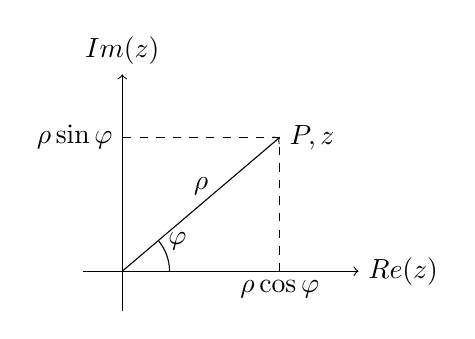
\begin{tikzpicture}\draw[->](-.5,0)--(3,0) node[right]{$\operatorname{Re}(z)$};\draw[->](0,-.5)--(0,2.5) node[above]{$\operatorname{Im}(z)$};\draw[->](0,0)--(2,1.7) node[right]{$P,z$} node[midway,above]{$\rho$};\draw[dashed](2,0) node[below]{$\rho\cos\varphi$}--(2,1.7)--(0,1.7) node[left]{$\rho\sin\varphi$};\draw(.6,0) arc(0:40:.6) node[right]{$\varphi$};\end{tikzpicture}\end{center}
\[z=\rho\cos\varphi+i\rho\sin\varphi=\rho(\cos\varphi+i\sin\varphi).\]
% Pagina originale 10
\pagina{10}
\[\rho=\sqrt{a^2+b^2}=\sqrt{\rho^2\cos^2\varphi+\rho^2\sin^2\varphi}=\sqrt{\rho^2}\sqrt{\cos^2\varphi+\sin^2\varphi}=|\rho|=\rho.\]
\[\begin{cases}\rho\cos\varphi=x,\\\rho\sin\varphi=y\end{cases}\implies
\begin{cases}\rho=x/\cos\varphi,\\\rho=y/\sin\varphi\end{cases}\implies\frac{x}{\cos\varphi}=\frac y{\sin\varphi}\implies\tan\varphi=\frac yx.\]
$\varphi=\arctan(y/x)$, con la scelta del quadrante:
\[\varphi=\begin{cases}\pi/2&x=0\land y>0,\\-\pi/2&x=0\land y<0,\\\arctan(y/x)&x>0,\\\arctan(y/x)\pm\pi&x<0.\end{cases}\]
\tit{Argomento e argomento principale}
Ogni numero complesso ha un argomento (escluso lo zero), che è l'angolo che si forma con l'asse delle ascisse.
\[z=(\rho,\operatorname{Arg}(z)+2k\pi).\]
$\operatorname{Arg}(z)$ è l'argomento principale, in $(-\pi,\pi]$.
\[\arg(z)=\operatorname{Arg}(z)+2k\pi,\qquad k\in\Z.\]
% Pagina originale 11
\pagina{11}
\tit{Prodotto in forma polare (o trigonometrica)}
\[\cos(\alpha\pm\beta)=\cos\alpha\cos\beta\mp\sin\alpha\sin\beta,\qquad
\sin(\alpha\pm\beta)=\sin\alpha\cos\beta\pm\sin\beta\cos\alpha.\]
\begin{align*}z_1z_2&=\rho_1\rho_2[\cos\varphi_1\cos\varphi_2+i\cos\varphi_1\sin\varphi_2+i\sin\varphi_1\cos\varphi_2-\sin\varphi_1\sin\varphi_2]\\
&=\rho_1\rho_2[\cos(\varphi_1+\varphi_2)+i\sin(\varphi_1+\varphi_2)].\end{align*}
\[\frac{z_1}{z_2}=\frac{\rho_1}{\rho_2}[\cos(\varphi_1-\varphi_2)+i\sin(\varphi_1-\varphi_2)].\]
\tit{Potenza (formula di De Moivre)}
\[\forall z\in\C:\quad z^n=\rho^n(\cos(n\varphi)+i\sin(n\varphi)).\]
\tit{Forma esponenziale (formula di Eulero)}
\[e^{i\varphi}=\cos\varphi+i\sin\varphi,\quad e^{i\pi}=\cos\pi+i\sin\pi=-1\implies\boxed{e^{i\pi}+1=0}\quad\text{(identità di Eulero)}.\]
\[\forall\varphi\in\R:\ |e^{i\varphi}|=1.\]
\tit{Radice $n$-esima di un numero complesso}
\[\sqrt[n]{w}=\sqrt[n]{|w|}\left(\cos\frac{\operatorname{Arg}(w)+2k\pi}{n}+i\sin\frac{\operatorname{Arg}(w)+2k\pi}{n}\right),\quad k=0,1,2,\ldots,n-1.\]
% Pagina originale 12
\pagina{12}
\tit{Osservazioni sulla forma esponenziale}
$|e^{i\theta}|=1$, $\forall\theta\in\R$ (anche $\forall\theta\in(-\pi,\pi]$).
$Ke^{i\theta}$ rappresenta tutti i numeri complessi; $K=|z|$, $\theta=\operatorname{Arg}(z)$.
\[K=e^{\ln K}\implies Ke^{i\theta}=e^{\ln K}e^{i\theta}=e^{\ln K+i\theta}=e^{m+i\theta}.\]
$me^{i\theta}$ con $m<0$ non è forma esponenziale: $m>0$ perché $m=|z|$.
\tit{Osservazioni sul modulo}
\[\forall z_1,z_2\in\C:\quad |z_1z_2|=|z_1||z_2|.\]
\tit{Disuguaglianza triangolare}
\[\forall z_1,z_2\in\C:\quad |z_1+z_2|\le |z_1|+|z_2|.\]
\begin{center}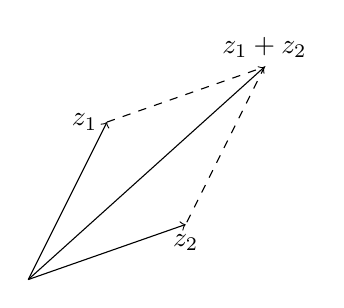
\begin{tikzpicture}\draw[->](0,0)--(1,2) node[left]{$z_1$};\draw[->](0,0)--(2,0.7) node[below]{$z_2$};\draw[->](0,0)--(3,2.7) node[above]{$z_1+z_2$};\draw[dashed](1,2)--(3,2.7)--(2,.7);\end{tikzpicture}\end{center}
$|z_1|+|z_2|=|z_1+z_2|$ se $z_1=kz_2$ con $k\in\R$ ($z_1$ ha stesso argomento di $z_2$).
\nota{Il manoscritto scrive $k\in\R$, senza specificarne la positività; è conservato.}
% Pagina originale 13
\pagina{13}
\tit{2 --- Funzioni}
$A\xrightarrow{\text{legge funzionale}}B$: $A$ è l'insieme di partenza (dominio); $B$ l'insieme di arrivo.
\[f:A\subset\R\to\R,\qquad y=f(x),\quad x\in A,\quad y\in\R.\]
$y$ è la variabile dipendente, $x$ la variabile indipendente.
\tit{Immagine di una funzione}
Sia $f:A\subset\R\to\R$ e $B\subset A$. Si chiama immagine mediante $f$ di $B$:
\[f(B):=\{y\in\R\mid\exists x\in B:\ y=f(x)\}.\]
$f(A)=\operatorname{Im}f$ (immagine della funzione = codominio).
\tit{Controimmagine di una funzione}
Sia $f:A\to C$ e $B\subset C$.
\[f^{-1}(B):=\{x\in A\mid f(x)\in B\}.\]
Se $f(x)=b\implies x\in f^{-1}(b)$.
Se $f$ non è iniettiva (esempio $y=x^2$), $f^{-1}(x)$ non è un singleton.
Esempio: $f^{-1}(1)=\{1,-1\}$.
% Pagina originale 14
\pagina{14}
\tit{Suriettività}
Sia $f:A\to B$. $f$ è suriettiva se $f(A)=B$.
Osservazione: una funzione può diventare suriettiva modificandone l'insieme di arrivo:
$f^*:A\to f(A)$ è suriettiva (restrizione del codominio).
\tit{Iniettività}
Sia $f:A\to B$. $f$ è iniettiva se (questi tre punti sono equivalenti):
\begin{enumerate}\item $\forall x_1,x_2\in A$, $x_1\ne x_2\implies f(x_1)\ne f(x_2)$.
\item $\forall b\in f(A)\ \exists!\bar x\in A:\ f(\bar x)=b$.
\item $\forall b\in f(A):f^{-1}(b)$ è un singleton (ha un solo elemento).
\end{enumerate}
\tit{Biettività o invertibilità}
Sia $f:A\to B$. $f$ è biettiva e invertibile se
\[\forall b\in f(A)\ \exists!\bar x\in A:f(\bar x)=b\quad\land\quad f(A)=B\]
\[\implies\forall b\in B\ \exists!\bar x\in A:f(\bar x)=b.\]
% Pagina originale 15
\pagina{15}
\tit{Funzione inversa}
Sia $f:A\to B$ invertibile. Esiste un'unica $f^{-1}:B\to A$, con
$f^{-1}(x)=y\in A$ tale che $f(y)=x$.
\tit{Restrizione dell'insieme di partenza}
Sia $f:A\to B$, $C\subset A$. Esiste $f|_C:C\to B$ tale che
$f|_C(x)=f(x)$ per ogni $x\in C$. $f|_C$ è detta restrizione di $f$ in $C$.
\tit{Funzione composta}
Siano $f:A\to B$, $g:C\to D$, $f(A)\subset C$. La funzione $g\circ f:A\to D$ è tale che
\[(g\circ f)(x)=g(f(x)),\quad\forall x\in A;\qquad g(f(x))\in D.\]
Esempio: $f(x)=x+1$, $g(x)=x^3$.
\[g\circ f=g(f(x))=g(x+1)=(x+1)^3,\qquad f\circ g=f(g(x))=f(x^3)=x^3+1.\]
$g\circ f\ne f\circ g$.
$(\R[x],\circ)$ è una legge di composizione interna (è un gruppo non abeliano).
\begin{itemize}\item Associativa: $f\circ(g\circ h)=(f\circ g)\circ h$.
\item Non commutativa: $g\circ f\ne f\circ g$.
\item Elemento neutro: $f(x)=x$.
\item Simmetrico: $g\circ g^{-1}=x$.
\end{itemize}
\nota{La qualificazione ``gruppo non abeliano'' è quella del manoscritto.}
% Pagina originale 16
\pagina{16}
\tit{Invertibilità di una funzione}
Sia $f:A\to B$. $f$ è invertibile se esiste $f^{-1}$ (ammette un'inversa):
\[\exists g:B\to A:\ g\circ f=i_A\land f\circ g=i_B,\]
\[g(f(x))=x\quad(A\to A),\qquad f(g(x))=x\quad(B\to B).\]
\tit{3 --- $f$ è invertibile $\iff f$ è biettiva}
\[f(x)=b\iff x=f^{-1}(b),\quad\text{perché}\quad f^{-1}(f(x))=f^{-1}(b),\quad x=f^{-1}(b).\]
\tit{Operazioni tra funzioni}
Sia $\mathcal F(A,\R):=\{f:A\to\R\mid f\text{ funzione}\}$, $A\subset\R$.
$\mathcal F$ è l'insieme di tutte le funzioni in $\R$.
\[f_1+f_2\in\mathcal F(A,\R),\quad(f_1+f_2)(x)=f_1(x)+f_2(x).\]
\[f_1f_2\in\mathcal F(A,\R),\quad(f_1f_2)(x)=f_1(x)f_2(x).\]
% Pagina originale 17
\pagina{17}
\tit{Tipi di funzione}
$f:A\to B$ è costante se $x\in A\mapsto\bar b\in B$.
$f:A\to B$ è identità se $x\in A\mapsto x\in A$.
Costante: $f(x)=K$, $K\in\R$; identità: $f(x)=x$.
\tit{Funzione potenza}
$f(x)=x^n$, $n\in\N$.
\[\begin{array}{c|l}n=0&f(x)=1\text{ (costante)}\\n=1&f(x)=x\text{ (identità)}\\n=2&f(x)=x^2\text{ (parabola)}\\n=3&f(x)=x^3\\\vdots&\vdots\end{array}\]
\begin{center}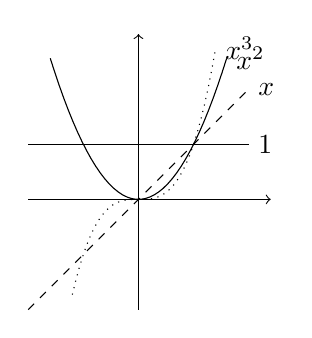
\begin{tikzpicture}[scale=.7]\draw[->](-2,0)--(2.4,0);\draw[->](0,-2)--(0,3);\draw[dashed](-2,-2)--(2,2) node[right]{$x$};\draw[domain=-1.6:1.6,samples=40]plot(\x,{\x*\x}) node[right]{$x^2$};\draw[dotted,domain=-1.2:1.4,samples=40]plot(\x,{\x*\x*\x}) node[right]{$x^3$};\draw(-2,1)--(2,1) node[right]{$1$};\end{tikzpicture}\end{center}
\tit{Monomio di una variabile}
$x\in\R\mapsto a_nx^n$, $a_n\in\R$, $n\in\N^*$.
\tit{Polinomio}
$p:\R\to\R$,
\[p(x)=a_0+a_1x+a_2x^2+a_3x^3+\cdots+a_nx^n=\sum_{i=0}^na_ix^i=a_ix^i\quad\text{(notazione di Einstein)}.\]
Se $a_n\ne0$, $n$ è il grado di $p$.
% Pagina originale 18
\pagina{18}
\tit{Funzioni lineari e affini}
$f(x)=ax$ è lineare; additiva: $f(x_1+x_2)=f(x_1)+f(x_2)$.
$f(x)=ax+K$, $K\ne0$, è affine.
\tit{Zeri di una funzione}
$f:A\to\R$, $Z_f:=\{x\in A\mid f(x)=0\}$.
\tit{Reciproco di una funzione}
$f:A\to\R$, $A\setminus Z_f:=\{x\in A\mid f(x)\ne0\}$.
\[\frac1f:A\setminus Z_f\to\R,\qquad\left(\frac1f\right)(x)=\frac1{f(x)}.\]
\tit{Rapporto tra funzioni}
$f_1,f_2\in\mathcal F(A,\R)$.
\[\frac{f_1}{f_2}:A\setminus Z_{f_2}\to\R,\qquad\left(\frac{f_1}{f_2}\right)(x)=\frac{f_1(x)}{f_2(x)},\qquad\frac{f_1}{f_2}:=f_1\frac1{f_2}.\]
\tit{Funzione razionale}
$f:\R\setminus Z_{p_2}\to\R$, $p_1,p_2:\R\to\R$, $f(x)=p_1(x)/p_2(x)$.
% Pagina originale 19
\pagina{19}
\tit{Funzione pari}
$f:A\to\R$, $\forall x\in A$ anche $-x\in A$; $f(-x)=f(x)$.
Esempi grafici: $|x|$, $\cos x$.
\tit{Funzione dispari}
$f:A\to\R$, $\forall x\in A:-x\in A$;
$f(-x)=-f(x)$ oppure $f(x)=-f(-x)$.
Esempi grafici: $x^3$, $\sin x$.
\tit{Funzione periodica}
$f:A\to\R$; $\exists t>0$ tale che $\forall x\in A:x+t\in A$.
\[f(x)=f(x+kt),\qquad\forall k\in\Z,\quad\forall x\in A;\qquad t\text{ periodo}.\]
\begin{center}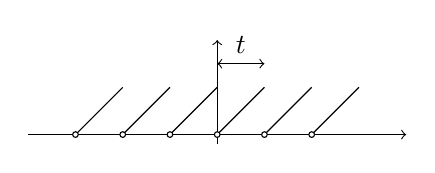
\begin{tikzpicture}[scale=.6]\draw[->](-4,0)--(4,0);\draw[->](0,-.2)--(0,2);\foreach \a in {-3,-2,-1,0,1,2}{\draw(\a,0)--(\a+1,1);\draw[fill=white](\a,0) circle(.06);}\draw[<->](0,1.5)--(1,1.5) node[midway,above]{$t$};\end{tikzpicture}\end{center}
\tit{Monotonia}
Sia $f:A\to\R$, $A\subset\R$, $B\subset A$.
\begin{itemize}\item $f$ è crescente in $B$ se $\forall x_1,x_2\in B$, $x_1<x_2:f(x_1)\le f(x_2)$.
\item $f$ è strettamente crescente in $B$ se $\forall x_1,x_2\in B$, $x_1<x_2:f(x_1)<f(x_2)$.
\item $f$ è decrescente in $B$ se $\forall x_1,x_2\in B$, $x_1<x_2:f(x_1)\ge f(x_2)$.
\end{itemize}
% Pagina originale 20
\pagina{20}
\tit{4 --- $f$ strettamente monotona $\implies f$ iniettiva}
Ipotesi: $f:A\to\R$, per $x_1<x_2$, $f(x_1)\ne f(x_2)$.
Tesi: $\forall x_1,x_2\in A$, $x_1\ne x_2$, $f(x_1)\ne f(x_2)$.
Dimostrazione: $x_1<x_2\implies x_1\ne x_2$.
\tit{5 --- $f,g$ monotone (stesso tipo) $\implies f+g$ monotona}
Ipotesi: $f,g:A\to\R$, $\forall x_1,x_2\in A$, $x_1<x_2$,
$f(x_1)\le f(x_2)$ e $g(x_1)\le g(x_2)$.
Tesi: $f+g:A\to\R$; $x_1<x_2\implies(f+g)(x_1)\le(f+g)(x_2)$.
Dimostrazione:
\begin{align*}&\forall x_1,x_2\in A,\ x_1<x_2:\quad f(x_1)\le f(x_2)\land g(x_1)\le g(x_2)\\
&\implies f(x_1)+g(x_1)\le f(x_2)+g(x_2)\\
&\implies(f+g)(x_1)\le(f+g)(x_2).
\end{align*}
Dimostrazione analoga per $f+g$ strettamente monotona se almeno una delle due lo è.
\tit{Prodotto di funzioni monotone}
$f,g$ monotone (stesso tipo), $f(x),g(x)>0$ per ogni $x\implies fg$ monotona.
Proposizione: siano $f:A\to\R$, $g:B\to\R$, $A\cap B\ne\varnothing$, $f,g$ monotone,
$f(x),g(x)>0$ per ogni $x\in A\cap B\implies fg$ monotona.
Grafici: $x^2$ crescente su $[0,+\infty)$, decrescente su $(-\infty,0]$; $x$ crescente.
% Pagina originale 21
\pagina{21}
Osservazioni: $x\cdot(-x)=-x^2$; $x\cdot x=x^2$; $x^2\cdot x=x^3$.
$C=$ crescente; $D=$ decrescente; $+=$ funzione positiva; $-=$ funzione negativa.
\[\begin{array}{c|c|c}f&g&fg\\\hline C-&C-&C+\\C-&C+&D+\\D+&D+&D+\\D+&D-&C+\end{array}\]
\nota{La tabella riproduce le sigle del manoscritto, comprese le indicazioni di segno presenti.}
\tit{6 --- $f$ monotona $\implies1/f$ monotona di tipo opposto}
Ipotesi: $f:A\to\R$, $\forall x_1,x_2\in A$, $x_1<x_2:f(x_1)\le f(x_2)$.
Tesi: $\forall x_1,x_2\in A\setminus Z_f$, $x_1<x_2:(1/f)(x_1)\ge(1/f)(x_2)$.
Dimostrazione:
\[f(x_1)\le f(x_2)\implies\frac1{f(x_1)}\ge\frac1{f(x_2)}\implies(1/f)(x_1)\ge(1/f)(x_2).\]
\nota{L'originale non esplicita qui l'ipotesi che la funzione mantenga il segno.}
\tit{7 --- $f$ strettamente monotona $\implies f^{-1}$ strettamente monotona con stesso tipo}
Ipotesi: $f:A\to\R$, $x_1<x_2\implies f(x_1)<f(x_2)$.
Tesi: $f^{-1}:f(A)\to A$, $x_1<x_2\implies f^{-1}(x_1)<f^{-1}(x_2)$.
Dimostrazione per assurdo: esistano $x_1,x_2\in f(A)$, $x_1<x_2$, tali che
$f^{-1}(x_1)\ge f^{-1}(x_2)$. $f^{-1}$ è iniettiva, quindi
$f^{-1}(x_1)>f^{-1}(x_2)$. Sono elementi di $A$, quindi
\[f(f^{-1}(x_1))>f(f^{-1}(x_2))\implies\boxed{x_1>x_2!}\]
% Pagina originale 22
\pagina{22}
\tit{8 --- Monotonia di funzioni composte}
Proposizione: $f:A\to B$, $g:C\to D$, $f(A)\subset C$.
\[\begin{array}{c|c|c|c}f&g&f\circ g&g\circ f\\\hline\nearrow&\nearrow&\nearrow&\nearrow\\\nearrow&\searrow&\searrow&\searrow\\\searrow&\nearrow&\searrow&\searrow\\\searrow&\searrow&\nearrow&\nearrow\end{array}\]
Ipotesi: $\forall x_1,x_2\in A$, $x_1<x_2:f(x_1)\ge f(x_2)$ (decrescente);
$\forall x_1,x_2\in C$, $x_1<x_2:g(x_1)\le g(x_2)$ (crescente).
Tesi: $\forall x_1,x_2\in A$, $x_1<x_2:g(f(x_1))\ge g(f(x_2))$.
Dimostrazione: $x_1<x_2\implies f(x_1)\ge f(x_2)$, e $f(x_1),f(x_2)\in f(A)\subset C$.
Per la monotonia di $g$, $g(f(x_1))\ge g(f(x_2))$.
% Pagina originale 23
\pagina{23}
\tit{Successione}
Una successione è una funzione con variabile discreta (in $\N$ oppure in $N\subset\N$).
$n\in\N$, $n\ge n_0\mapsto a_n\in\R$.
Notazioni: $\{a_n\}_{n\ge n_0}$, $(a_n)_{n\ge n_0}$, $a_n$.
\begin{enumerate}\item $n\in\N\mapsto i^n\in\C$.
\item $n\in\N\mapsto n\in\N$.
\end{enumerate}
Gli insiemi d'arrivo $B\subseteq\C$: (1) e (2) sono successioni numeriche.
$(1-1/n)_{n\ge1}$ ha come immagine l'insieme $A$:
\[A=\{x\in\R:\exists n\in\N^*,\ x=1-1/n\}=\{0,1/2,2/3,3/4,4/5,5/6,\ldots\}.\]
$(1-1/n)_{n\ge1}$ è la restrizione in $\N$ di $f(x)=1-1/x$, $f:[1,+\infty)\to\R$.
\[\{(-1)^n\}_{n\in\N}=\{\cos(n\pi)\}_{n\in\N},\qquad\{\sin(n\pi)\}_{n\in\N}=0\quad\forall n\in\N.\]
% Pagina originale 24
\pagina{24}
\tit{Successione estratta o sottosuccessione}
$(a_n)_{n\in N\subset\N}$ è una successione.
$(a_n)_{n\in S\subset N\subset\N}$, con $S\ne\varnothing$, è una successione estratta da $(a_n)_{n\in N}$ (o sottosuccessione).
\tit{Monotonia nelle successioni}
$(a_n)_{n\ge n_0}$ è monotona crescente se
\[\forall n_1,n_2\in\N,\quad n_0\le n_1\le n_2:\ a_{n_1}\le a_{n_2}.\]
Basta dire che $\forall n\in\N$, $n\ge n_0:a_n\le a_{n+1}$.
\tit{Maggiorante di una funzione}
$f:A\to\R$. $M$ è maggiorante per $f$ se
\[\forall x\in A:M\ge f(x)\iff\forall y\in f(A):M\ge y.\]
\tit{Minorante di una funzione}
$f:A\to\R$. $m$ è minorante per $f$ se
\[\forall x\in A:m\le f(x)\iff\forall y\in f(A):m\le y.\]
% Pagina originale 25
\pagina{25}
\tit{Funzione limitata}
$f:A\to\R$ è limitata se
\[\exists m,M\in\R:\forall x\in A,\ m\le f(x)\le M,\]
oppure $\exists K\in\R^+$ tale che $\forall x\in A:|f(x)|\le K$.
\begin{center}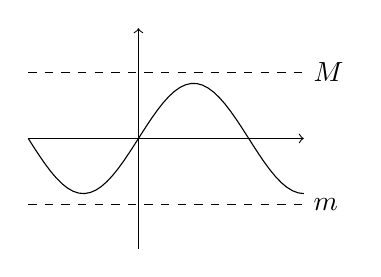
\begin{tikzpicture}[scale=.7]\draw[->](-2,0)--(3,0);\draw[->](0,-2)--(0,2);\draw[dashed](-2,1.2)--(3,1.2) node[right]{$M$};\draw[dashed](-2,-1.2)--(3,-1.2) node[right]{$m$};\draw[domain=-2:3,samples=50]plot(\x,{sin(90*\x)});\end{tikzpicture}\end{center}
\tit{Relazione d'ordine tra funzioni}
$f,g:A\to\R$; $f\le g:=\forall x\in A:f(x)\le g(x)$.
\tit{Modulo di una funzione}
$f:A\to\R$; $|f|:A\to[0,+\infty)$, $|f|(x):=|f(x)|$, $\forall x\in A$.
\tit{Massimo di una funzione}
$f:A\to\R$; $\exists x_M\in A$ tale che $\forall x\in A:f(x_M)\ge f(x)$.
$x_M$ è punto di massimo, $f(x_M)$ valore di massimo.
\tit{Massimo forte}
$\exists!x_M\in A$ tale che $\forall x\in A\setminus\{x_M\}:f(x_M)>f(x)$.
% Pagina originale 26
\pagina{26}
\tit{Massimo relativo o locale}
$f:A\to\R$, $x_0\in A$, $\delta>0$.
$x_0$ è punto di massimo relativo se
\[\forall x\in(x_0-\delta,x_0+\delta)\cap A,\quad f(x_0)\ge f(x).\]
\tit{Inf e sup di una funzione}
$f:A\to\R$.
\[\Lambda=\sup f\iff\begin{cases}\forall x\in A:f(x)\le\Lambda,\\\forall\varepsilon>0\ \exists\bar x\in A:f(\bar x)>\Lambda-\varepsilon;\end{cases}\]
\[\lambda=\inf f\iff\begin{cases}\forall x\in A:f(x)\ge\lambda,\\\forall\varepsilon>0\ \exists\bar x\in A:f(\bar x)<\lambda+\varepsilon.\end{cases}\]
\tit{Intorno}
Sia $x_0\in\R$.
\[\mathcal I(x_0):=\{I\subset\R\mid\exists\delta>0:\ I=(x_0-\delta,x_0+\delta)\}.\]
\[\mathcal I(+\infty):=\{I\subset\R\mid\exists a\in\R:\ I=(a,+\infty)\},\quad
\mathcal I(-\infty):=\{I\subset\R\mid\exists a\in\R:\ I=(-\infty,a)\}.\]
\tit{Punto di accumulazione}
$x_0\in\overline\R$ è punto di accumulazione per $A\subset\R$ se
\[\forall U\in\mathcal I(x_0):\quad(U\cap A)\setminus\{x_0\}\ne\varnothing.\]
$D(A):=\{x\in\overline\R\mid x\text{ è punto di accumulazione}\}$.
% Pagina originale 27
\pagina{27}
\tit{Punto isolato}
$x_0\in\R$ è punto isolato in $A\subset\R$ se
$\exists U\in\mathcal I(x_0)$ tale che $(U\cap A)\setminus\{x_0\}=\varnothing$;
$x_0\notin D(A)$.
\tit{$+\infty$ punto di accumulazione in un insieme illimitato superiormente}
Ipotesi: $A=(a,+\infty)$.
Tesi: $\forall U\in\mathcal I(+\infty):(U\cap A)\setminus\{+\infty\}\ne\varnothing$.
Dimostrazione: $U=(b,+\infty)$ con $b\in\R$.
\[(b,+\infty)\cap(a,+\infty)=\begin{cases}(a,+\infty)&a\ge b,\\(b,+\infty)&b>a.\end{cases}\]
Sia $c=\begin{cases}a&a\ge b,\\b&b>a.\end{cases}$ Allora $(c,+\infty)\ne\varnothing$.
% Pagina originale 28
\pagina{28}
\tit{3 --- Limiti}
$f:A\to\R$, $x_0\in D(A)$ e $l\in\overline\R$.
$\lim_{x\to x_0}f(x)=l$, oppure $f(x)\xrightarrow{x\to x_0}l$, se e solo se
\[\forall V\in\mathcal I(l)\ \exists U\in\mathcal I(x_0):\quad\forall x\in(U\cap A)\setminus\{x_0\},\ f(x)\in V.\]
Nel disegno a sinistra $\lim_{x\to x_0}f(x)\ne l$; a destra $\lim_{x\to x_0}f(x)=l$: ogni $f(x)\in V$ per ogni $x\in U$.
\tit{Definizione con intervalli (algebrica)}
$x_0\in D(A)$, $l\in\R$:
\[\forall\varepsilon>0\ \exists\delta>0:\ \forall x\in[A\cap(x_0-\delta,x_0+\delta)]\setminus\{x_0\},\quad f(x)\in(l-\varepsilon,l+\varepsilon).\]
$\varepsilon$ è il raggio dell'intorno di $l$, $\delta$ il raggio dell'intorno di $x_0$.
\[\forall\varepsilon>0\ \exists\delta>0:\quad\forall x\in A,\ 0<|x-x_0|<\delta\implies|f(x)-l|<\varepsilon.\]
% Pagina originale 29
\pagina{29}
\begin{itemize}
\item $x_0\in D(A)\cap\R$, $l=+\infty$:
$\forall a\in\R\ \exists\delta_a>0$ tale che $\forall x\in A$, $0<|x-x_0|<\delta_a\implies f(x)>a$.
\item $x_0\in D(A)\cap\R$, $l=-\infty$:
$\forall a\in\R\ \exists\delta_a>0$ tale che $\forall x\in A$, $0<|x-x_0|<\delta_a\implies f(x)<a$.
\item $x_0\in D(A)$, $x_0=+\infty$, $l=+\infty$:
$\forall a\in\R\ \exists\delta_a\in\R$ tale che $\forall x\in A$, $x>\delta_a\implies f(x)>a$.
\item $x_0\in D(A)$, $x_0=-\infty$, $l=-\infty$:
$\forall a\in\R\ \exists\delta_a\in\R$ tale che $\forall x\in A$, $x<\delta_a\implies f(x)<a$.
\item $x_0\in D(A)$, $x_0=+\infty$, $l\in\R$:
$\forall\varepsilon>0\ \exists\delta_\varepsilon\in\R$ tale che $\forall x\in A$, $x>\delta_\varepsilon\implies|f(x)-l|<\varepsilon$.
\end{itemize}
% Pagina originale 30
\pagina{30}
\tit{Continuità}
$f:A\to\R$, $x_0\in A$. $f$ è continua in $x_0$ se
\[\forall V\in\mathcal I(f(x_0))\ \exists U\in\mathcal I(x_0):\forall x\in A\cap U,\quad f(x)\in V.\]
\[\forall\varepsilon>0\ \exists\delta_\varepsilon>0:\quad\forall x\in A,\ |x-x_0|<\delta_\varepsilon\implies|f(x)-f(x_0)|<\varepsilon.\]
\tit{Osservazioni sulla continuità}
\begin{enumerate}\item Un punto isolato è continuo.
\item Se $x_0\in D(A)$ e $f$ continua in $x_0$, allora $\lim_{x\to x_0}f(x)=f(x_0)$.
\end{enumerate}
\tit{$f$ continua in un insieme}
$f:A\to\R$, $B\subset A$. $f$ continua in $B\iff f$ continua in $x$ per ogni $x\in B$.
\tit{Limiti nelle successioni}
\[\lim_nx_n=l\in\overline\R\iff\forall V\in\mathcal I(l)\ \exists\nu\in\N:\forall n\ge\nu,\ x_n\in V.\]
Cioè $x_n\in V$ risulta definitivamente. Esempio grafico: $\lim_n1/n=0$.
% Pagina originale 31
\pagina{31}
\tit{9 --- $\{x_n\}$ monotona $\implies\exists\lim_nx_n=\sup(x_n)\in\overline\R$ (o inf)}
Ipotesi: $\forall n\in\N:a_n\le a_{n+1}$.
\begin{itemize}\item $\sup(x_n)=+\infty\implies\lim_nx_n=+\infty$.
$\forall a\in\R\ \exists\nu\in\N:x_\nu>a$.
Dimostrazione: $\forall a\in\R\ \exists\nu\in\N$ tale che $\forall n>\nu:x_n\ge x_\nu>a$, per crescenza.
\item $\sup(x_n)=\Lambda\in\R\implies\lim_nx_n=\Lambda$.
$\forall\varepsilon>0\ \exists\nu\in\N:\Lambda\ge x_\nu\ge\Lambda-\varepsilon$.
Dimostrazione: $\forall\varepsilon>0\ \exists\nu\in\N$ tale che $\forall n\in\N$, $n>\nu$:
$\Lambda\ge x_n\ge x_\nu>\Lambda-\varepsilon$, per crescenza.
\end{itemize}
\tit{Convergenza e divergenza nelle successioni}
$\lim_nx_n=l\in\R\implies x_n$ converge a $l$.
$\lim_nx_n\in\{+\infty,-\infty\}\implies x_n$ diverge a $\pm\infty$.
\tit{Convergenza e divergenza nelle funzioni}
$\lim_{x\to x_0}f(x)=l\in\R\implies f$ è convergente in $x_0$.
Se il limite è $\pm\infty$, $f$ è divergente in $x_0$.
\tit{Infinito e infinitesimo}
$\lim_{x\to x_0\in\overline\R}f(x)=\pm\infty\implies f$ è un infinito per $x_0$.
$\lim_{x\to x_0\in\overline\R}f(x)=0\implies f$ è un infinitesimo per $x_0$.
% Pagina originale 32
\pagina{32}
\tit{Teorema ponte}
$f:A\to\R$, $x_0\in D(A)$.
\[\exists\lim_{x\to x_0}f(x)=l\in\overline\R\iff
\forall(x_n)_{n\ge n_0}\subset A\setminus\{x_0\},\ x_n\to x_0:\quad f(x_n)\to l.\]
\tit{Non esistenza del limite di $\sin x$ usando il teorema ponte}
Prendo due successioni che tendono a $-\infty$:
\[x_n^{(1)}=(-n\pi)_{n\in\N},\qquad x_n^{(2)}=(\pi/2-2n\pi)_{n\in\N}.\]
$x_n^{(1)}\to-\infty$, $x_n^{(2)}\to-\infty$.
$\sin(x_n^{(1)})=0$ per ogni $n\in\N$; $\sin(x_n^{(2)})=1$ per ogni $n\in\N$.
I valori sono diversi, quindi $\nexists\lim_{x\to-\infty}\sin x$.
\nota{Il titolo del manoscritto indica $x\to+\infty$, mentre il calcolo scritto usa $-\infty$.}
\tit{Limite da destra e da sinistra}
$f:A\to\R$, $x_0\in D^+(A)$, $l\in\overline\R$.
$\lim_{x\to x_0^+}f(x)=l$ se
\[\forall V\in\mathcal I(l)\ \exists\delta>0:\quad\forall x\in A\cap(x_0,x_0+\delta),\ f(x)\in V.\]
% Pagina originale 33
\pagina{33}
\tit{Punto di accumulazione a destra o a sinistra}
$A\subset\R$, $x_0\in\R$ è punto di accumulazione a destra se
$\forall\delta>0:(x_0,x_0+\delta)\cap A\ne\varnothing$;
cioè $\forall U\in\mathcal I^+(x_0):A\cap U\ne\varnothing\implies x_0\in D^+(A)$.
\[\mathcal I^+(x_0):=\{I\subset\R\mid\exists\delta>0:\ I=(x_0,x_0+\delta)\},\]
\[\mathcal I^-(x_0):=\{I\subset\R\mid\exists\delta>0:\ I=(x_0-\delta,x_0)\}.\]
\tit{Osservazioni sui limiti da destra o da sinistra}
Se $x_0\in D^+(A)\setminus D^-(A)$: non esiste il limite da sinistra, il limite da destra è il limite.
\tit{10 --- Equivalenza tra limite e limiti laterali}
\[\exists\lim_{x\to x_0}f(x)=l\in\overline\R\iff
\exists\lim_{x\to x_0^-}f(x)=l\land\exists\lim_{x\to x_0^+}f(x)=l.\]
$(\Rightarrow)$ Ipotesi: $\forall\varepsilon>0\ \exists\delta>0$ tale che $\forall x\in A$, $0<|x-x_0|<\delta:\ |f(x)-l|<\varepsilon$.
Tesi: la stessa disuguaglianza vale per $x\in(x_0,x_0+\delta)$ e per $x\in(x_0-\delta,x_0)$.
Dimostrazione: $x\in(x_0-\delta,x_0+\delta)$, $x\ne x_0$, equivale a
$x\in(x_0-\delta,x_0)\cup(x_0,x_0+\delta)$, su cui $|f(x)-l|<\varepsilon$.
% Pagina originale 34
\pagina{34}
\tit{11 --- Limite delle funzioni monotone}
Sia $f:A\to\R$, $f$ monotona in $A$, $x_0\in D^+(A)$.
Se $f$ è crescente:
\[\exists\lim_{x\to x_0^+}f(x)=\inf_{x\in A\cap(x_0,+\infty)}f(x),\qquad
\exists\lim_{x\to x_0^-}f(x)=\sup_{x\in A\cap(-\infty,x_0)}f(x).\]
Se $f$ è decrescente, rispettivamente $\sup$ e $\inf$ sugli stessi insiemi.
\tit{Corollario}
$f:(a,b)\to\R$, monotona crescente in $(a,b)$:
\[\exists\lim_{x\to a^+}f(x)=\inf f(x),\qquad\exists\lim_{x\to b^-}f(x)=\sup f(x).\]
$f:[a,b]\to\R$:
\[\exists\lim_{x\to a^+}f(x)=\inf_{x\in(a,b]}f(x)\ne\inf_{x\in[a,b]}f(x)=f(a),\]
\[\exists\lim_{x\to b^-}f(x)=\sup_{x\in[a,b)}f(x)\ne\sup_{x\in[a,b]}f(x)=f(b).\]
\nota{Il manoscritto usa $\ne$ nelle ultime righe: l'uguaglianza può invece verificarsi quando non vi è salto agli estremi.}
\begin{center}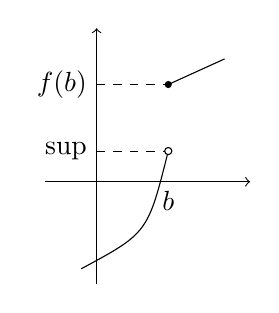
\begin{tikzpicture}[scale=.65]\draw[->](-1,0)--(3,0);\draw[->](0,-2)--(0,3);\draw(-.3,-1.7)..controls(1,-1)..(1.4,.6);\draw(1.4,1.9)--(2.5,2.4);\draw[dashed](0,.6)--(1.4,.6);\draw[dashed](0,1.9)--(1.4,1.9);\draw[fill=white](1.4,.6)circle(.07);\fill(1.4,1.9)circle(.07);\node[below]at(1.4,0){$b$};\node[left]at(0,.6){$\sup$};\node[left]at(0,1.9){$f(b)$};\end{tikzpicture}\end{center}
% Pagina originale 35
\pagina{35}
\tit{12 --- Teorema della permanenza del segno (funzione con limite)}
Ipotesi: $f:A\to\R$, $x_0\in D(A)$, $\exists\lim_{x\to x_0}f(x)=l>0$.
Tesi: $\exists U\in\mathcal I(x_0):\forall x\in(A\cap U)\setminus\{x_0\},f(x)>0$.
Dimostrazione: $\forall V\in\mathcal I(l)\ \exists U\in\mathcal I(x_0)$ tale che $\forall x\in(A\cap U)\setminus\{x_0\}:f(x)\in V$.
Prendo $V\subset(0,+\infty)$, essendo $l>0$: quindi $\exists\varepsilon>0$ tale che $\forall x\in(l-\varepsilon,l+\varepsilon):x>0$.
Quindi $\exists U\in\mathcal I(x_0)$ tale che $\forall x\in(A\cap U)\setminus\{x_0\}:f(x)\in V\implies f(x)>0$.
\tit{13 --- Teorema della permanenza del segno (funzione continua)}
Ipotesi: $f:A\to\R$, $x_0\in D(A)$, $f(x_0)>0$, $f\in C^0(\{x_0\})$.
Tesi: $\exists U\in\mathcal I(x_0)$ tale che $\forall x\in A\cap U:f(x)>0$.
Dimostrazione: $\forall V\in\mathcal I(f(x_0))\ \exists U\in\mathcal I(x_0)$ tale che $\forall x\in A\cap U:f(x)\in V$.
Prendo $V\subset(0,+\infty)$; quindi $\exists U\in\mathcal I(x_0)$ tale che $\forall x\in A\cap U:f(x)\in V\implies f(x)>0$.
% Pagina originale 36
\pagina{36}
\tit{14 --- Conseguenza del teorema della permanenza del segno}
Ipotesi: $f,g:I\to\R$, $x_0\in\mathring I$, $f(x)<g(x)$ in un intorno di $x_0$, cioè $\exists U\in\mathcal I(x_0)$ tale che $\forall x\in I\cap U:f(x)<g(x)$.
Tesi: $\lim_{x\to x_0}f(x)\le\lim_{x\to x_0}g(x)$.
Dimostrazione per assurdo: $\lim_{x\to x_0}f(x)=l_f$, $\lim_{x\to x_0}g(x)=l_g$.
Per assurdo $l_f>l_g\implies l_f-l_g>0$.
\[h(x):=f(x)-g(x),\qquad\exists\lim_{x\to x_0}h(x)=\lim_{x\to x_0}(f(x)-g(x)).\]
$\lim h(x)>0\implies\exists U\in\mathcal I(x_0)$ tale che $\forall x\in(I\cap U)\setminus\{x_0\}:h(x)>0\implies f(x)>g(x)$: assurdo!
\tit{Operazioni tra limiti}
$f,g:A\to\R$, $x_0\in D(A)$, $\exists\lim f(x)=l_f\in\overline\R$, $\exists\lim g(x)=l_g\in\overline\R$.
Allora $\exists\lim(f+g)=l_f+l_g\in\overline\R$ e $\exists\lim(fg)=l_fl_g\in\overline\R$, quando le operazioni sono definite.
Nelle tabelle $\square$ indica forma indeterminata; $a,b$ indicano numeri reali finiti.
\[\begin{array}{c|rrrr}+&+\infty&-\infty&0&b\\\hline+\infty&+\infty&\square&+\infty&+\infty\\-\infty&\square&-\infty&-\infty&-\infty\\0&+\infty&-\infty&0&b\\a&+\infty&-\infty&a&a+b\end{array}\quad\begin{array}{c|rrrrr}\cdot&+\infty&-\infty&0&b>0&b<0\\\hline+\infty&+\infty&-\infty&\square&+\infty&-\infty\\-\infty&-\infty&+\infty&\square&-\infty&+\infty\\0&\square&\square&0&0&0\\a>0&+\infty&-\infty&0&ab&ab\\a<0&-\infty&+\infty&0&ab&ab\end{array}\]
% Pagina originale 37
\pagina{37}
\tit{15 --- Teorema degli zeri}
Ipotesi: $f:[a,b]\to\R$, $f\in C^0([a,b])$, $f(a)f(b)<0$.
Tesi: $\exists x_0\in(a,b):f(x_0)=0$.
Dimostrazione con metodo di bisezione. $a=a_0$, $b=b_0$, $c_0:=(a_0+b_0)/2$.
Se $f(c_0)=0$, $x_0=c_0$. Se $f(c_0)\ne0$:
\[f(a_0)f(c_0)<0\implies\begin{cases}a_1=a_0\\b_1=c_0\end{cases},\qquad f(c_0)f(b_0)<0\implies\begin{cases}a_1=c_0\\b_1=b_0\end{cases},\quad c_1:=\frac{a_1+b_1}{2}.\]
Si creano due successioni $\{a_n\}$ e $\{b_n\}$ limitate, con $a\le a_n<b$ e $a<b_n\le b$, $\forall n\in\N$.
$\{a_n\}$ è crescente e $\{b_n\}$ decrescente.
$\{a_n\}$ crescente perché $a_n\le a_{n+1}$: $a_{n+1}=a_n$ oppure $a_{n+1}=(a_n+b_n)/2$, con $b_n>a_n$, quindi $a_{n+1}=(a_n+b_n)/2>2a_n/2=a_n$.
$\{b_n\}$ decrescente perché $b_n\ge b_{n+1}$: $b_{n+1}=b_n$ oppure $b_{n+1}=(a_n+b_n)/2$, con $b_n>a_n$, quindi $b_{n+1}=(a_n+b_n)/2<2b_n/2=b_n$.
% Pagina originale 38
\pagina{38}
La successione $\{b_n-a_n\}=\{(b-a)/2^n\}$.
\[\lim_n\frac{b-a}{2^n}=0\implies\lim_n(b_n-a_n)=l_2-l_1=0\implies l_2=l_1.\]
Sia $x_0:=l_1=l_2$. $\lim_{x\to x_0}f(x)=f(x_0)$, poiché $f$ è continua.
Utilizzando il teorema ponte:
\[\lim_{x\to x_0}f(x)=f(x_0)\implies f(a_n)\to f(x_0),\quad f(b_n)\to f(x_0).\]
$f(a_n)f(b_n)<0\implies f(x_0)f(x_0)\le0$, sfruttando il teorema della permanenza del segno.
$[f(x_0)]^2\le0\iff f(x_0)=0$.
\tit{Osservazioni sul teorema degli zeri}
1) Se $f:A\to\R$, $A$ insieme e $\exists[a,b]\subset A:f(a)f(b)<0$, allora $\exists x_0\in(a,b):f(x_0)=0$.
\nota{L'osservazione presuppone la continuità della restrizione a $[a,b]$.}
2) Ci consente di stabilire se $f(x)$ ha zeri ($f(x)=0$ ha soluzioni).
% Pagina originale 39
\pagina{39}
3) Analogamente ci consente di stabilire se $f(x)=g(x)$ ha soluzioni ($h(x):=f(x)-g(x)$, $h(x)=0$).
4) Tutte le ipotesi sono necessarie.
Esempio: $f(x)=\begin{cases}1&x\ge0\\-1&x<0.\end{cases}$.
$f(a)f(b)<0$, ma $\nexists x_0\in(a,b):f(x_0)=0$.
\begin{center}\begin{tikzpicture}[scale=.6]\draw[->](-3,0)--(3,0);\draw[->](0,-2)--(0,2);\draw(-3,-1)--(0,-1);\draw(0,1)--(3,1);\draw[fill=white](0,-1)circle(.08);\fill(0,1)circle(.08);\node[below]at(-1,0){$a$};\node[below]at(1,0){$b$};\end{tikzpicture}\end{center}
\tit{16 --- Corollario del teorema degli zeri}
Ipotesi: $f:(a,b)\to\R$, $f\in C^0((a,b))$, $a,b\in\overline\R$.
Se $\exists\lim_{x\to a^+}f(x)=l_a$ e $\exists\lim_{x\to b^-}f(x)=l_b$, $l_al_b<0$.
Tesi: $\exists x_0\in(a,b):f(x_0)=0$.
Dimostrazione. [Passaggio segnato ``inutile'' nell'originale:] $\exists\lim_{x\to a^+}f(x)=l_a\implies\exists V_a\in\mathcal I^+(a)$ tale che $\forall x\in V_a\cap(a,b):f(x)\in U_a\in\mathcal I(l_a)$.
$l_al_b<0\implies\exists V_a\in\mathcal I^+(a),V_b\in\mathcal I^-(b)$ tali che $\forall x_a\in V_a\cap(a,b),x_b\in V_b\cap(a,b):f(x_a)f(x_b)<0$.
Prendendo $\bar x_a\in V_a\cap(a,b)$, $\bar x_b\in V_b\cap(a,b)$ posso applicare il teorema degli zeri alla restrizione $f|_{[\bar x_a,\bar x_b]}\in C^0([\bar x_a,\bar x_b])$.
$f(\bar x_a)f(\bar x_b)<0\implies\exists x_0\in(\bar x_a,\bar x_b):f(x_0)=0$, e $(\bar x_a,\bar x_b)\subset(a,b)$.
% Pagina originale 40
\pagina{40}
\tit{Osservazioni sul corollario}
Vale anche per intervalli del tipo $[a,b)$, $[a,b]$, $(a,b]$.
\[\lim_{x\to a}f(x)\,f(b)<0\implies\lim_{x\to a}f(x)\lim_{x\to b}f(x)<0,\]
essendo $f\in C^0((a,b])$.
\tit{17 --- Teorema dei valori intermedi}
Ipotesi: $f:A\to\R$, $f\in C^0(A)$, $I\subset A$, $I$ intervallo.
Tesi: $f(I)$ intervallo, cioè $\forall y_1,y_2\in f(I):\forall y\in(y_1,y_2):y\in f(I)$.
Di conseguenza $\forall y\in f(I)\ \exists\bar x\in I:f(\bar x)=y$.
Dimostrazione: $y_1,y_2\in f(I)$, $y_1<y_2$, $x_1,x_2\in I$, $x_1\ne x_2$, con $f(x_1)=y_1$, $f(x_2)=y_2$.
Supponiamo $x_1<x_2$; $[x_1,x_2]\subset I$. Prendo $y$ con $y_1<y<y_2$.
$h(x):=f(x)-y$, $h\in C^0([x_1,x_2])$, perché $f\in C^0([x_1,x_2])$ e $y$ costante.
\[h(x_1)=y_1-y<0,\qquad h(x_2)=y_2-y>0\implies h(x_1)h(x_2)<0.\]
Quindi $\exists\bar x\in(x_1,x_2)\subset I:h(\bar x)=0\implies f(\bar x)-y=0\implies f(\bar x)=y$.
\begin{center}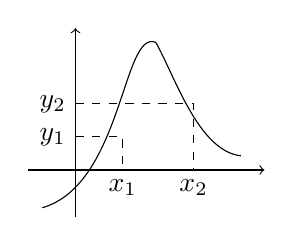
\begin{tikzpicture}[scale=.6]\draw[->](-1,0)--(4,0);\draw[->](0,-1)--(0,3);\draw(-.7,-.8)..controls(1,-.3)and(1,3)..(1.7,2.7)..controls(2.1,2)and(2.6,.4)..(3.5,.3);\draw[dashed](0,.7)--(1,.7)--(1,0);\draw[dashed](0,1.4)--(2.5,1.4)--(2.5,0);\node[left]at(0,.7){$y_1$};\node[left]at(0,1.4){$y_2$};\node[below]at(1,0){$x_1$};\node[below]at(2.5,0){$x_2$};\end{tikzpicture}\end{center}
Lo stesso grafico traslato verticalmente di $-y$ rappresenta $h(x)$: $h(x_1)<0$, $h(x_2)>0$, e lo zero è $\bar x$.
% Pagina originale 41
\pagina{41}
\tit{18 --- Teorema di Weierstrass}
Ipotesi: $f:[a,b]\to\R$, $f\in C^0([a,b])$.
Tesi: $f$ ha minimo e massimo: $\exists\min f,\max f\in\R$.
\tit{Teorema dei valori intermedi + teorema di Weierstrass}
Ipotesi: $f:[a,b]\to\R$, $f\in C^0([a,b])$.
Tesi: $f([a,b])=[m,M]$, con $m=\min f$, $M=\max f$.
\tit{Funzioni elementari}
Affine: $f(x)=ax+b$. Lineare: $f(x)=ax$.
Potenza: $f(x)=x^n$, $n>1$, $n\in\N$.
Esponenziali: $f(x)=a^x$, $a>0$, $a\ne1$; dominio $\R$, $f(\R)=\R_+^*$.
Logaritmiche: $f(x)=\log_a x$, $a>0$, $a\ne1$; dominio $x>0$, $f(\R_+^*)=\R$.
\begin{center}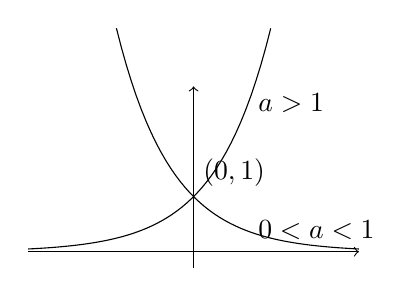
\begin{tikzpicture}[scale=.7]\draw[->](-3,0)--(3,0);\draw[->](0,-.3)--(0,3);\draw[domain=-3:1.4,samples=50]plot(\x,{exp(\x)});\draw[domain=-1.4:3,samples=50]plot(\x,{exp(-\x)});\node[above right]at(0,1){$(0,1)$};\node[right]at(1,2.7){$a>1$};\node[right]at(1,.4){$0<a<1$};\end{tikzpicture}\quad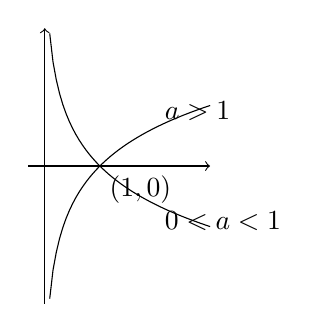
\begin{tikzpicture}[scale=.7]\draw[->](-.3,0)--(3,0);\draw[->](0,-2.5)--(0,2.5);\draw[domain=.09:3,samples=50]plot(\x,{ln(\x)});\draw[domain=.09:3,samples=50]plot(\x,{-ln(\x)});\node[below right]at(1,0){$(1,0)$};\node[right]at(2,1){$a>1$};\node[right]at(2,-1){$0<a<1$};\end{tikzpicture}\end{center}
% Pagina originale 42
\pagina{42}
\tit{Trigonometriche}
$P=(\cos\alpha,\sin\alpha)$ sulla circonferenza $\mathcal C:x^2+y^2=1$, centro $C_{\mathcal C}=(0,0)$, raggio $r_{\mathcal C}=1$.
\begin{center}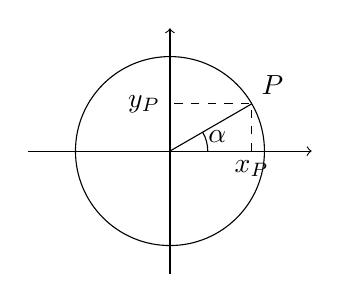
\begin{tikzpicture}[scale=1.2]\draw[->](-1.5,0)--(1.5,0);\draw[->](0,-1.3)--(0,1.3);\draw(0,0)circle(1);\draw(0,0)--(.866,.5);\draw[dashed](.866,0)--(.866,.5)--(0,.5);\draw(.4,0)arc(0:30:.4);\node at(.5,.15){$\alpha$};\node[above right]at(.866,.5){$P$};\node[below]at(.866,0){$x_P$};\node[left]at(0,.5){$y_P$};\end{tikzpicture}\end{center}
Prima identità fondamentale: $\cos^2\alpha+\sin^2\alpha=1$, da $x^2+y^2=1$ per ogni $(x,y)\in\mathcal C$.
Seconda identità fondamentale: $\tan\alpha=\sin\alpha/\cos\alpha$.
\tit{Trigonometriche inverse}
\begin{center}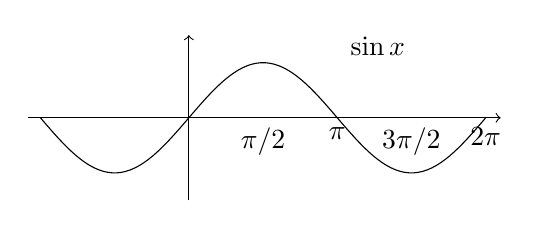
\begin{tikzpicture}[xscale=.6,yscale=.7]\draw[->](-3.4,0)--(6.6,0);\draw[->](0,-1.5)--(0,1.5);\draw[domain=-3.14:6.28,samples=100]plot(\x,{sin(\x r)});\node at(4,1.3){$\sin x$};\node[below]at(1.57,0){$\pi/2$};\node[below]at(3.14,0){$\pi$};\node[below]at(4.71,0){$3\pi/2$};\node[below]at(6.28,0){$2\pi$};\end{tikzpicture}\quad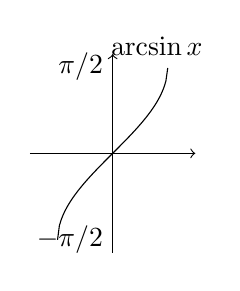
\begin{tikzpicture}[scale=.7]\draw[->](-1.5,0)--(1.5,0);\draw[->](0,-1.8)--(0,1.8);\draw[domain=-1:1,samples=60]plot(\x,{asin(\x)/180*pi});\node[above]at(.8,1.6){$\arcsin x$};\node[left]at(0,1.57){$\pi/2$};\node[left]at(0,-1.57){$-\pi/2$};\end{tikzpicture}

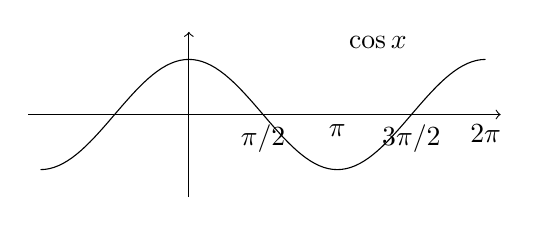
\begin{tikzpicture}[xscale=.6,yscale=.7]\draw[->](-3.4,0)--(6.6,0);\draw[->](0,-1.5)--(0,1.5);\draw[domain=-3.14:6.28,samples=100]plot(\x,{cos(\x r)});\node at(4,1.3){$\cos x$};\node[below]at(1.57,0){$\pi/2$};\node[below]at(3.14,0){$\pi$};\node[below]at(4.71,0){$3\pi/2$};\node[below]at(6.28,0){$2\pi$};\end{tikzpicture}\quad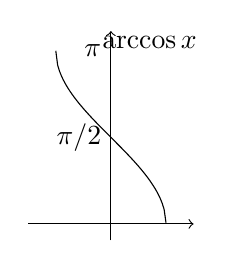
\begin{tikzpicture}[scale=.7]\draw[->](-1.5,0)--(1.5,0);\draw[->](0,-.3)--(0,3.5);\draw[domain=-1:1,samples=60]plot(\x,{acos(\x)/180*pi});\node[above]at(.7,3){$\arccos x$};\node[left]at(0,3.14){$\pi$};\node[left]at(0,1.57){$\pi/2$};\end{tikzpicture}

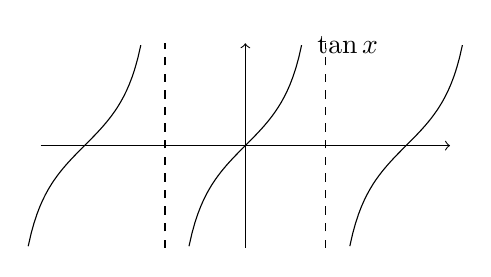
\begin{tikzpicture}[scale=.65]\draw[->](-4,0)--(4,0);\draw[->](0,-2)--(0,2);\foreach \s in {-3.1416,0,3.1416}{\draw[domain=-1.1:1.1,samples=40]plot({\x+\s},{tan(\x r)});}\foreach \s in {-1.57,1.57}{\draw[dashed](\s,-2)--(\s,2);}\node[above]at(2,1.6){$\tan x$};\end{tikzpicture}\quad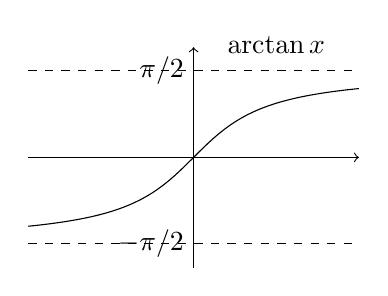
\begin{tikzpicture}[scale=.7]\draw[->](-3,0)--(3,0);\draw[->](0,-2)--(0,2);\draw[domain=-3:3,samples=60]plot(\x,{atan(\x)/180*pi});\draw[dashed](-3,1.57)--(3,1.57);\draw[dashed](-3,-1.57)--(3,-1.57);\node[above]at(1.5,1.7){$\arctan x$};\node[left]at(0,1.57){$\pi/2$};\node[left]at(0,-1.57){$-\pi/2$};\end{tikzpicture}\end{center}
% Pagina originale 43
\pagina{43}
\begin{center}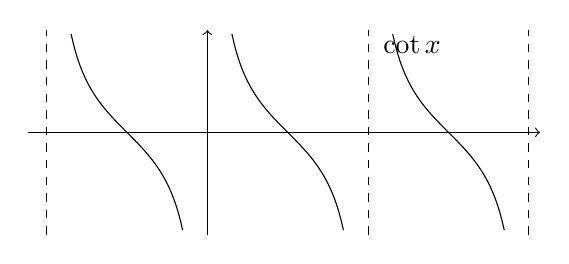
\begin{tikzpicture}[scale=.65]\draw[->](-3.5,0)--(6.5,0);\draw[->](0,-2)--(0,2);\foreach \s in {-3.1416,0,3.1416}{\draw[domain=.48:2.66,samples=50]plot({\x+\s},{1/tan(\x r)});}\foreach \s in {-3.14,0,3.14,6.28}{\draw[dashed](\s,-2)--(\s,2);}\node at(4,1.7){$\cot x$};\end{tikzpicture}\quad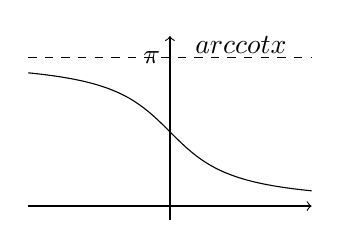
\begin{tikzpicture}[scale=.6]\draw[->](-3,0)--(3,0);\draw[->](0,-.3)--(0,3.6);\draw[domain=-3:3,samples=60]plot(\x,{pi/2-atan(\x)/180*pi});\draw[dashed](-3,3.14)--(3,3.14);\node at(1.5,3.4){$\operatorname{arccot}x$};\node[left]at(0,3.14){$\pi$};\end{tikzpicture}\end{center}
\tit{Angoli notevoli}
\[\cos(x-\pi/2)=\sin x,\qquad\sin(x+\pi/2)=\cos x,\]
\[\cos(2x)=\cos^2x-\sin^2x,\qquad\sin(2x)=2\cos x\sin x.\]
\tit{Tangente}
$OPH$ e $OTA$ sono simili, quindi $\overline{HP}/\overline{HO}=\overline{TA}/\overline{OA}$, cioè $\sin x/\cos x=\overline{TA}/1$; quindi $\overline{TA}=\sin x/\cos x=\tan x$.
\begin{center}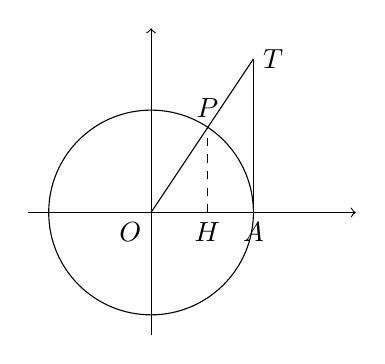
\begin{tikzpicture}[scale=1.3]\draw[->](-1.2,0)--(2,0);\draw[->](0,-1.2)--(0,1.8);\draw(0,0)circle(1);\draw(1,0)--(1,1.5);\draw(0,0)--(1,1.5);\draw[dashed](.55,0)--(.55,.83);\node[below left]at(0,0){$O$};\node[below]at(.55,0){$H$};\node[below]at(1,0){$A$};\node[above]at(.55,.83){$P$};\node[right]at(1,1.5){$T$};\end{tikzpicture}\end{center}
\tit{Iperboliche}
\[\sinh x:=\frac{e^x-e^{-x}}2,\qquad\cosh x:=\frac{e^x+e^{-x}}2.\]
$\sinh(-x)=-\sinh x$, $\cosh(-x)=\cosh x$; $\sinh0=0$, $\cosh0=1$.
$\forall x\in\R:\cosh^2x-\sinh^2x=1$.
\nota{La prima identità di parità è corretta a penna nel manoscritto.}
\begin{center}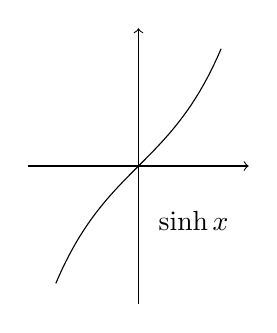
\begin{tikzpicture}[scale=.7]\draw[->](-2,0)--(2,0);\draw[->](0,-2.5)--(0,2.5);\draw[domain=-1.5:1.5,samples=50]plot(\x,{(exp(\x)-exp(-\x))/2});\node at(1,-1){$\sinh x$};\end{tikzpicture}\quad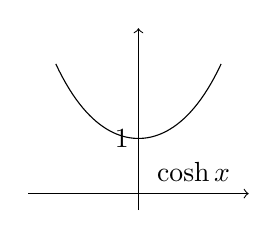
\begin{tikzpicture}[scale=.7]\draw[->](-2,0)--(2,0);\draw[->](0,-.3)--(0,3);\draw[domain=-1.5:1.5,samples=50]plot(\x,{(exp(\x)+exp(-\x))/2});\node[left]at(0,1){$1$};\node at(1,.4){$\cosh x$};\end{tikzpicture}\quad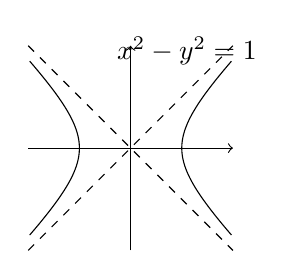
\begin{tikzpicture}[scale=.65]\draw[->](-2,0)--(2,0);\draw[->](0,-2)--(0,2);\draw[dashed](-2,-2)--(2,2);\draw[dashed](-2,2)--(2,-2);\draw[domain=-1.3:1.3,samples=50]plot({(exp(\x)+exp(-\x))/2},{(exp(\x)-exp(-\x))/2});\draw[domain=-1.3:1.3,samples=50]plot({-(exp(\x)+exp(-\x))/2},{(exp(\x)-exp(-\x))/2});\node at(1.1,1.9){$x^2-y^2=1$};\end{tikzpicture}\end{center}
% Pagina originale 44
\pagina{44}
\tit{Iperboliche inverse}
\[y=\operatorname{sett}\sinh x=\ln(x+\sqrt{x^2+1}),\qquad y=\operatorname{sett}\cosh x=\ln(x+\sqrt{x^2-1}).\]
Nomi: settore seno iperbolico ($\sinh^{-1}$), settore coseno iperbolico ($\cosh^{-1}$).
\nota{Il manoscritto scrive ``$\sinh x=y\iff y=\ln(x+\sqrt{x^2+1})$'' e analogamente per cosh: le variabili risultano scambiate.}
\begin{center}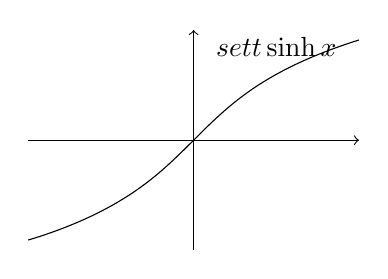
\begin{tikzpicture}[scale=.7]\draw[->](-3,0)--(3,0);\draw[->](0,-2)--(0,2);\draw[domain=-3:3,samples=60]plot(\x,{ln(\x+sqrt(\x*\x+1))});\node at(1.5,1.7){$\operatorname{sett}\sinh x$};\end{tikzpicture}\quad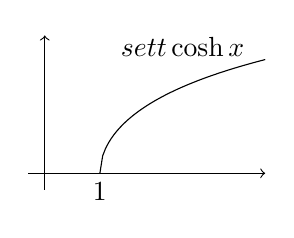
\begin{tikzpicture}[scale=.7]\draw[->](-.3,0)--(4,0);\draw[->](0,-.3)--(0,2.5);\draw[domain=1:4,samples=60]plot(\x,{ln(\x+sqrt(\x*\x-1))});\node[below]at(1,0){$1$};\node at(2.5,2.3){$\operatorname{sett}\cosh x$};\end{tikzpicture}\end{center}
\tit{19 --- Teorema di unicità del limite}
$f:A\to\R$, $x_0\in D(A)$, $\exists\lim_{x\to x_0}f(x)=l\in\overline\R\implies l$ è unico.
Dimostrazione per assurdo: $\lim_{x\to x_0}f(x)=l_1,l_2$, con $l_1\ne l_2$.
Allora $\forall V_1\in\mathcal I(l_1)\ \exists U_1\in\mathcal I(x_0)$ tale che $\forall x\in(A\cap U_1)\setminus\{x_0\}:f(x)\in V_1$;
e $\forall V_2\in\mathcal I(l_2)\ \exists U_2\in\mathcal I(x_0)$ tale che $\forall x\in(A\cap U_2)\setminus\{x_0\}:f(x)\in V_2$.
Quindi $\exists U\in\mathcal I(x_0)$ tale che $\forall x\in(A\cap U)\setminus\{x_0\}:f(x)\in V_1\cap V_2=\varnothing$: assurdo!
$U=U_1\cap U_2\ne\varnothing$ (due intorni dello stesso punto non hanno intersezione vuota).
\nota{Per ottenere l'assurdo si scelgono $V_1,V_2$ disgiunti, possibile perché $l_1\ne l_2$.}
% Pagina originale 45
\pagina{45}
\tit{Rapporto tra limiti}
$f_1,f_2:A\to\R$, $Z_{f_2}=\{x\in A:f_2(x)=0\}$.
$f_1/f_2:A\setminus Z_{f_2}\to\R$, $(f_1/f_2)(x):=f_1(x)/f_2(x)$.
\[x_0\in D(A\setminus Z_{f_2})\implies\exists\lim_{x\to x_0}\frac{f_1(x)}{f_2(x)}=\frac{\lim f_1(x)}{\lim f_2(x)}=\frac{l_1}{l_2}.\]
$\square$ indica forme indeterminate. $a>0$, $b<0$, $c>0$, $d<0$.
\[\begin{array}{c|rrrrr}/&+\infty&-\infty&0&c&d\\\hline+\infty&\square&\square&+\infty&+\infty&-\infty\\-\infty&\square&\square&-\infty&-\infty&+\infty\\0&0&0&\square&0&0\\a&0&0&\pm\infty&a/c&a/d\\b&0&0&\pm\infty&b/c&b/d\end{array}\]
\nota{Il segno di un quoziente con denominatore tendente a zero dipende dal lato con cui questo tende a zero.}
\tit{Limite per eccesso e per difetto}
$\lim_{x\to x_0}f(x)=l^+$: si dice che $f$ tende ad $l$ per eccesso se
\[\forall V\in\mathcal I(l)\ \exists U\in\mathcal I(x_0):\forall x\in(A\cap U)\setminus\{x_0\},\ f(x)\in V\cap(l,+\infty).\]
$\lim_{x\to x_0}f(x)=l^-$: si dice che $f$ tende ad $l$ per difetto se
\[\forall V\in\mathcal I(l)\ \exists U\in\mathcal I(x_0):\forall x\in(A\cap U)\setminus\{x_0\},\ f(x)\in V\cap(-\infty,l).\]
% Pagina originale 46
\pagina{46}
\tit{20 --- Teorema del doppio confronto}
$f,g,h:A\to\R$, $x_0\in D(A)$.
$\exists U\in\mathcal I(x_0)$ tale che $f\le g\le h$ per ogni $x\in(U\cap A)\setminus\{x_0\}$.
$\exists\lim_{x\to x_0}f(x)=\lim_{x\to x_0}h(x)=l\in\R\implies\exists\lim_{x\to x_0}g(x)=l$.
Dimostrazione: $\exists\lim g(x)=l\iff\forall\varepsilon>0\ \exists\bar U\in\mathcal I(x_0)$ tale che $\forall x\in(\bar U\cap A)\setminus\{x_0\}:|g(x)-l|<\varepsilon$.
Fisso $\bar\varepsilon>0$: $\exists U_f,U_h\in\mathcal I(x_0)$ tali che
\[\forall x\in(U_f\cap A)\setminus\{x_0\}:|f(x)-l|<\bar\varepsilon,\quad\forall x\in(U_h\cap A)\setminus\{x_0\}:|h(x)-l|<\bar\varepsilon.\]
Sia $\bar U:=U_f\cap U_h\in\mathcal I(x_0)$ (intersecando anche con l'intorno in cui vale il confronto).
Allora $\forall x\in(\bar U\cap A)\setminus\{x_0\}$:
\[|f(x)-l|<\bar\varepsilon\land|h(x)-l|<\bar\varepsilon\implies l-\bar\varepsilon<f(x)<l+\bar\varepsilon\land l-\bar\varepsilon<h(x)<l+\bar\varepsilon.\]
\[l-\bar\varepsilon<f(x)\le g(x)\le h(x)<l+\bar\varepsilon\implies l-\bar\varepsilon<g(x)<l+\bar\varepsilon\implies|g(x)-l|<\bar\varepsilon.\]
% Pagina originale 47
\pagina{47}
\tit{21 --- Teorema del confronto}
$f,g:A\to\R$, $x_0\in D(A)$, $\exists U\in\mathcal I(x_0)$ tale che $f\le g$ per ogni $x\in(U\cap A)\setminus\{x_0\}$.
$\exists\lim_{x\to x_0}f(x)=+\infty\implies\exists\lim_{x\to x_0}g(x)=+\infty$.
\tit{22 --- Limite nullo e modulo}
$f:A\to\R$, $x_0\in D(A)$:
\[\exists\lim_{x\to x_0}f(x)=0\iff\exists\lim_{x\to x_0}|f(x)|=0.\]
Dimostrazione:
$\forall\varepsilon>0\ \exists\delta>0:\forall x\in A,\ 0<|x-x_0|<\delta:|f(x)-0|<\varepsilon$
equivalente a $\forall\varepsilon>0\ \exists\delta>0:\forall x\in A,\ 0<|x-x_0|<\delta:\bigl||f(x)|-0\bigr|<\varepsilon$,
poiché $|f(x)|=\bigl||f(x)|\bigr|$.
\nota{Il manoscritto omette $0<$ nelle due righe della definizione.}
\tit{Prodotto tra infinitesimo e limitato}
$f,g:A\to\R$, $x_0\in D(A)$, $\exists\lim_{x\to x_0}f(x)=0\in\R$, $\exists\lim_{x\to x_0}g(x)=l\in\R^*$.
Allora $\lim_{x\to x_0}f(x)g(x)=0$.
% Pagina originale 48
\pagina{48}
\tit{23 --- Teorema del limite delle funzioni composte}
$f:A\to\R$, $g:B\to\R$, $f(A)\subset B$.
$x_0\in D(A)$, $\exists\lim_{x\to x_0}f(x)=l\in\overline\R$;
$l\in D(B)$, $\exists\lim_{y\to l}g(y)=l_1\in\overline\R$.
$\exists U_1\in\mathcal I(x_0)$ tale che $\forall x\in(U_1\cap A)\setminus\{x_0\}:f(x)\ne l$ (oppure $g\in C^0(B)$).
Allora $\exists\lim_{x\to x_0}g\circ f=l_1$.
Dimostrazione: $\forall V\in\mathcal I(l_1)\ \exists U\in\mathcal I(x_0)$ tale che $\forall x\in(U\cap A)\setminus\{x_0\}:g(f(x))\in V$.
Fisso $\bar V\in\mathcal I(l_1)$.
$\exists W_1\in\mathcal I(l)$ tale che $\forall y\in(W_1\cap B)\setminus\{l\}:g(y)\in\bar V$.
$\exists U_W\in\mathcal I(x_0)$ tale che $\forall x\in(U_W\cap A)\setminus\{x_0\}:f(x)\in W_1$.
Quindi $g(f(x))\in\bar V$; ma se $g$ non è continua serve $f(x)\ne l$, quindi $x\in U_1$.
Pertanto $\forall x\in(U_W\cap U_1\cap A)\setminus\{x_0\}:g(f(x))\in\bar V$.
\nota{Nella riga per $y$ il manoscritto scrive $\setminus\{x_0\}$ al posto di $\setminus\{l\}$.}
% Pagina originale 49
\pagina{49}
\tit{24 --- Continuità di funzioni composte da funzioni continue}
$f:A\to\R$, $g:B\to\R$, $f(A)\subset B$, $f\in C^0(A)$, $g\in C^0(B)\implies g\circ f\in C^0(A)$.
Caso più generale: $C\subset A$, $f\in C^0(C)$, $g\in C^0(f(C))\implies g\circ f\in C^0(C)$.
\tit{Punti di discontinuità}
$f:A\to\R$, $x_0\in D(A)$, $x_0\in A$.
1) $x_0$ punto di discontinuità a salto (di I specie):
$x_0\in D^+(A)\cap D^-(A)$,
$\exists\lim_{x\to x_0^+}f(x)=l^+\in\R$, $\exists\lim_{x\to x_0^-}f(x)=l^-\in\R$, con $l^+\ne l^-$; salto $\sigma=|l^+-l^-|$.
2) $x_0$ punto di discontinuità di II specie: $x_0\in D(A)$ e almeno uno tra $\lim_{x\to x_0^-}f(x)$, $\lim_{x\to x_0^+}f(x)$ non esiste oppure è $\pm\infty$.
3) $x_0$ punto di discontinuità di III specie (eliminabile): $\exists\lim_{x\to x_0}f(x)\in\R$, diverso da $f(x_0)$.
% Pagina originale 50
\pagina{50}
\tit{Eliminazione di un punto di discontinuità di III specie}
$f:A\to\R$,
\[\widetilde f(x)=\begin{cases}f(x)&x\ne x_0,\\\lim_{x\to x_0}f(x)&x=x_0.\end{cases}\]
\begin{center}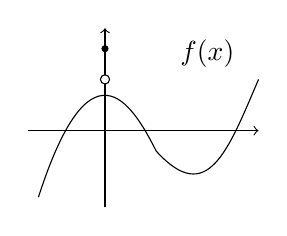
\begin{tikzpicture}[scale=.65]\draw[->](-1.5,0)--(3,0);\draw[->](0,-1.5)--(0,2);\draw(-1.3,-1.3)..controls(-.3,1.8)and(.5,.6)..(1,-.4)..controls(2,-1.5)and(2.4,-.4)..(3,1);\draw[fill=white](0,1)circle(.09);\fill(0,1.6)circle(.07);\node at(2,1.5){$f(x)$};\end{tikzpicture}\quad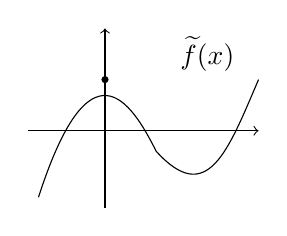
\begin{tikzpicture}[scale=.65]\draw[->](-1.5,0)--(3,0);\draw[->](0,-1.5)--(0,2);\draw(-1.3,-1.3)..controls(-.3,1.8)and(.5,.6)..(1,-.4)..controls(2,-1.5)and(2.4,-.4)..(3,1);\fill(0,1)circle(.07);\node at(2,1.5){$\widetilde f(x)$};\end{tikzpicture}\end{center}
\tit{Asintoti}
\tit{Asintoto verticale}
La retta $x=x_0$ è asintoto verticale se $\exists\lim_{x\to x_0}f(x)=\pm\infty$.
\tit{Asintoto orizzontale}
La retta $y=q\in\R$ è asintoto orizzontale se $\exists\lim_{x\to\pm\infty}f(x)=q\in\R$.
\tit{Asintoto obliquo}
La retta $y=mx+q$ è asintoto obliquo se $\exists\lim_{x\to\pm\infty}(f(x)-mx-q)=0$, con $m\ne0$, $m,q\in\R$.
\[m=\lim_{x\to\pm\infty}\frac{f(x)}x,\qquad q=\lim_{x\to\pm\infty}(f(x)-mx).\]
